\section{Systemtest med kendt input}
I dette afsnit vil det samlede system blive testet, så det er muligt at se, om systemet behandler dette input, som det forventes. På baggrund af disse målinger er det muligt at konkludere, om systemet virker. 

\subsection{Beskrivelse}
For at teste om det samlede system med et kendt input benyttes en funktionsgenerator, så der kan genereres et sinussignal på $500~Hz$ med en peak-peak-amplitude på $4~mV$. Sinussignalets frekvens og amplitude er nær ved, hvad der kan forventes af et filtreret EMG-signal. Outputtet fra sinussignalet er filtreret gennem lavpasfiltreret. 

Der foretages endnu en måling  samtidig for at test accelerometer-signalerne. Dette gøres ved at indsende to spændinger svarende til de to accelerometre. Denne varireres over tid, således at den overskrider de spændinger, der svarer til $90-180^{\circ}$.

Hele testen foretages i 10 sekunder og optages via mikrokontrolleren. Ud fra disse målinger, er det muligt at se effekten af systemets blokke, når de er sammensat ved at sammenligne input-signalet og outputtet af sinussignalet samt spændingerne for det samlede acclerometre. Resultaterne fra målingerne visualiseres i MATLAB. 


\subsection{Resultater af test}
Fra testen plottes og visualiseres systemets input af sinussignalet og outputtet fra det filtrerede signal, samt den omregnede spænding til en vinkel for begge de målte spændinger. Derudover er der plottet den digitale ouputsignal fra EMG-algoritmen. Resultaterne fremgår af \autoref{fig:test_kendtinput}. 

\begin{figure}[H]
\centering
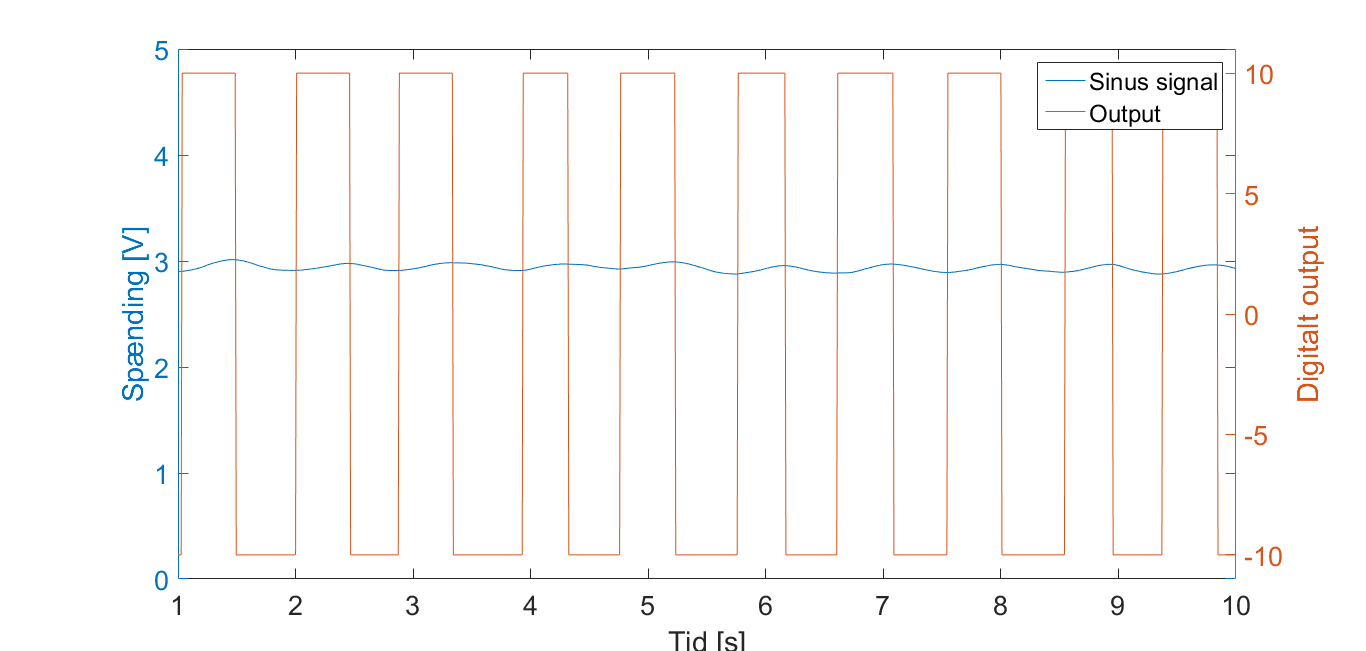
\includegraphics[width=0.4\textwidth]{figures/kontrol_test_sinus.jpg}
\caption{På den øverste figur, illustrer den blå graf inputsignalet svarende til en sinus på $500~Hz$ med en $V_{pp}$ på $4~mV$. Den røde graf illustrer sinussignalet som er filtreret, disse værdier er målt i spændingen, som det ses på den venstre Y-akse. Den gule graf viser den samlede spænding omregnet til en vinkel, hvilket fremgår af den højre Y-akse. På den nederste figur er den blå graf signalets digitale output i EMG-algoritmen}
\label{fig:test_kendtinput}
\end{figure}

På baggrund af målingerne for \autoref{fig:test_kendtinput} ses det at ved en stigende spænding svarende til $90-180^{\circ}$ vil vinklen stige, hvilket stemmer overens med forventningen. Det fremgår af grafen at ved en spænding svarende til omkring $180^{\circ}$, hvilket på grafen svarer til $175^{\circ}$ hvor den overskrider, hvorved grafen går i $-115^{\circ}$. I følge implementering skal signalet når det overstiger $180^{\circ}$ gå i $-200^{\circ}$. Disse faktorer er angiveligt fordi den ene spænding ikke har været tilsvarende, hvorved denne har været modsigende i forhold til beregningen af den samlede vinkel.

Det fremgår af \autoref{fig:test_kendtinput}, hvis der ses på EMGsignalet 


 findes lokale maksima- og minimapunkter. For at kunne udregne forsinkelsen sammenlignes forskellen mellem de lokale ekstrema, hvor der undersøges hvornår outputtet skifter spænding, altså differensen mellem lokale ekstrema og skift i outputspænding. Resultaterne for dette fremgår af \autoref{tab:sinus_ekstrema}.


\begin{table}[H]
\centering
\begin{tabular}{|c|c|c|}
\hline
\textbf{Ekstrema {[}s{]}} & \textbf{Output-skift {[}s{]}} & \textbf{Forsinkelse {[}s{]}} \\ \hline
3,0132                    & 2,8778                        & 0,1354                       \\ \hline
2,9922                    & 2,8859                        & 0,1063                       \\ \hline
2,9842                    & 2,8907                        & 0,0935                       \\ \hline
2,9777                    & 2,8939                        & 0,0838                       \\ \hline
2,9713                    & 2,9020                        & 0,0693                       \\ \hline
2,9713                    & 2,9101                        & 0,0612                       \\ \hline
2,9681                    & 2,9101                        & 0,0580                       \\ \hline
2,9681                    & 2,9117                        & 0,0564                       \\ \hline
2,9632                    & 2,9246                        & 0,0386                       \\ \hline
2,9568                    & 2,9278                        & 0,0290                       \\ \hline
\end{tabular}
\caption{Målt ekstrema, output-skift og differensen mellem disse, som fremgår som forsinkelse}
\label{tab:sinus_ekstrema}
\end{table}

Af \autoref{tab:sinus_ekstrema} fremgår det, at forsinkelsen fra inputsignalet registreres som en ændring  i output-signalet og er mellem $0,0290~s$ og $0,1354~s$. Ud fra dette er den gennemsnitlige forsinkelse beregnet til at være $0,07315~s$, hvilket svarer til omkring $73~ms$. 


\subsection{Konklusion}
.....